\documentclass[usenames,dvipsnames,tikz]{standalone}
%\usepackage{amsmath,amssymb}
%\usepackage{xcolor}
\colorlet{tBlue}{RoyalBlue!35!Cerulean}
\colorlet{tRed}{Red}
%\usepackage{tikz}
%\usepackage{standalone}
\begin{document}
	
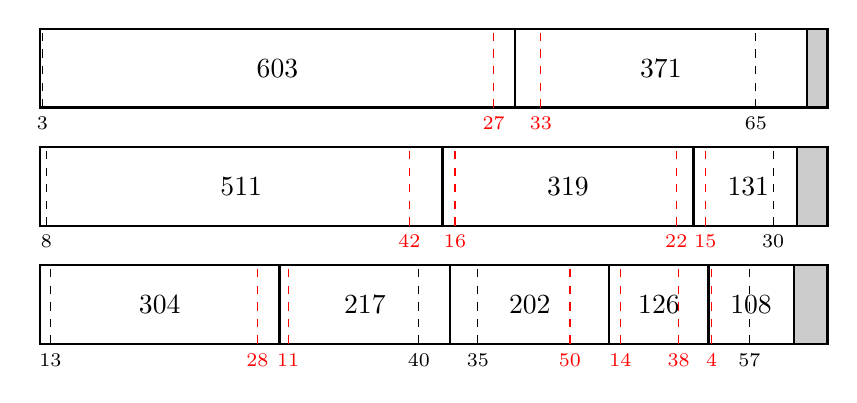
\begin{tikzpicture}
%\draw [help lines] (-1,-2) grid (11,5);
% 1=0.1, 2=0.15, 3=0.2, 4=0.25, 5=0.3
% 6 (3-27), 5 (8-42), 4 (33-65), 4 (16-22), 3 (13-28), 3 (11-40), 2 (35-50), 1 (15-30), 1 (14-38), 1 (4-57).


% BPP
\draw [thick] (0,0) rectangle (10,1); %bottom row
\draw [thick] (0,1.5) rectangle (10,2.5); %middle row
\draw [thick] (0,3) rectangle (10,4); %top row
%\draw [thick, white] (0,4.5) rectangle (10,5.5);
 
% Bottom row, 304, 217, 202, 126, 108 (13-28 X 11-40, 35-50 X 14-38 X 4-47)
\draw [thick] (3.04,0) -- (3.04,1);
\draw [thick] (5.21,0) -- (5.21,1);
\draw [thick] (7.23,0) -- (7.23,1);
\draw [thick] (8.49,0) -- (8.49,1);
\draw [thick, fill=black!20!white] (9.58,0) rectangle (10,1);

\node at (1.52, 0.5) {$304$};
\node at (4.125, 0.5) {$217$};
\node at (6.22, 0.5) {$202$};
\node at (7.86, 0.5) {$126$};
\node at (9.03, 0.5) {$108$};

\draw [dashed] (0.13,0) -- (0.13,1); 
\draw [dashed, tRed] (2.76,0) -- (2.76,1);
\node [below] at (0.13,0) {\scriptsize{$13$}};
\node [below] at (2.76,0) {\textcolor{tRed}{\scriptsize{$28$}}};

\draw [dashed, tRed] (3.15,0) -- (3.15,1);
\draw [dashed] (4.81,0) -- (4.81,1);
\node [below] at (3.15,0) {\textcolor{tRed}{\scriptsize{$11$}}};
\node [below] at (4.81,0) {\scriptsize{$40$}};

\draw [dashed] (5.56,0) -- (5.56,1);
\draw [dashed, tRed] (6.73,0) -- (6.73,1);
\node [below] at (5.56,0) {\scriptsize{$35$}};
\node [below] at (6.73,0) {\textcolor{tRed}{\scriptsize{$50$}}};

\draw [dashed, tRed] (7.37,0) -- (7.37,1);
\draw [dashed, tRed] (8.11,0) -- (8.11,1);
\node [below] at (7.37,0) {\textcolor{tRed}{\scriptsize{$14$}}};
\node [below] at (8.11,0) {\textcolor{tRed}{\scriptsize{$38$}}};

\draw [dashed, tRed] (8.53,0) -- (8.53,1);
\draw [dashed] (9.01,0) -- (9.01,1);
\node [below] at (8.53,0) {\textcolor{tRed}{\scriptsize{$4$}}};
\node [below] at (9.01,0) {\scriptsize{$57$}};

% Middle row, 511, 335, 131 (8-42 X 16-22 X 15-30)
\draw [thick] (5.11,1.5) -- (5.11,2.5);
\draw [thick] (8.3,1.5) -- (8.3,2.5);
\draw [thick, fill=black!20!white] (9.61,1.5) rectangle (10,2.5);

\node at (2.555, 2) {$511$};
\node at (6.705, 2) {$319$};
\node at (8.995, 2) {$131$};

\draw [dashed] (0.08,1.5) -- (0.08,2.5);
\draw [dashed, tRed] (4.69,1.5) -- (4.69,2.5);
\node [below] at (0.08,1.5) {\scriptsize{$8$}};
\node [below] at (4.69,1.5) {\textcolor{tRed}{\scriptsize{$42$}}};

\draw [dashed, tRed] (5.27,1.5) -- (5.27,2.5);
\draw [dashed, tRed] (8.08,1.5) -- (8.08,2.5);
\node [below] at (5.27,1.5) {\textcolor{tRed}{\scriptsize{$16$}}};
\node [below] at (8.08,1.5) {\textcolor{tRed}{\scriptsize{$22$}}};

\draw [dashed, tRed] (8.45,1.5) -- (8.45,2.5);
\draw [dashed] (9.31,1.5) -- (9.31,2.5);
\node [below] at (8.45,1.5) {\textcolor{tRed}{\scriptsize{$15$}}};
\node [below] at (9.31,1.5) {\scriptsize{$30$}};

% Top row, 603, 382 (3-27 X 33-65)
\draw [thick] (6.03,3) -- (6.03,4);
\draw [thick, fill=black!20!white] (9.74,3) rectangle (10,4);

\draw [dashed] (0.03,3) -- (0.03,4);
\draw [dashed, tRed] (5.76,3) -- (5.76,4);
\node [below] at (0.03,3) {\scriptsize{$3$}};
\node [below] at (5.76,3) {\textcolor{tRed}{\scriptsize{$27$}}};

\draw [dashed, tRed] (6.36,3) -- (6.36,4);
\draw [dashed] (9.09,3) -- (9.09,4);
\node [below] at (6.36,3) {\textcolor{tRed}{\scriptsize{$33$}}};
\node [below] at (9.09,3) {\scriptsize{$65$}};

\node at (3.015, 3.5) {$603$};
\node at (7.885, 3.5) {$371$};

%--------------------------



\end{tikzpicture}

\end{document}